\documentclass[12pt]{article}

\usepackage{fontspec}
\usepackage{ctex}
\usepackage{cite}
\usepackage{apacite}
\usepackage{setspace}
\usepackage{enumitem}
\usepackage{diagbox}
\usepackage{xcolor}
\usepackage{tabularx}
\usepackage{graphicx}
\usepackage[english]{babel}
\usepackage{cleveref}
\usepackage{float}
\usepackage{geometry}
\usepackage{tikz}
\usepackage{lastpage}
\usepackage{titlesec}
\usepackage{makecell}


\geometry{a4paper, left=2.5cm, right=2.5cm, top=2.5cm, bottom=1.25cm}

\setmainfont{Times New Roman}
\setmonofont{Consolas}

\setCJKmainfont[AutoFakeBold]{SimSun.ttc}

\newCJKfontfamily\hwzs{STZhongsong}[AutoFakeBold]
\newfontfamily\hwzseng{STZhongsong}[AutoFakeBold]
\newfontfamily\calibri{Calibri}
\newfontfamily\cambria{Cambria}

\newCJKfontfamily\hwxk{STXingkai}[AutoFakeBold]

\providecommand{\tightlist}{\setlength{\itemsep}{0pt}\setlength{\parskip}{0pt}}

\usepackage{url}
\urlstyle{rm}
\usepackage{xurl}

\renewcommand{\arraystretch}{1.5}

\usepackage{caption}
\captionsetup{labelfont=it, labelsep=period, font={stretch=1.2}}

\titleformat{\section}{\normalfont\bfseries\centering\zihao{-4}}{}{0pt}{}
\titleformat{\subsection}{\normalfont\bfseries\zihao{-4}\raggedright}{}{0pt}{}

\renewcommand\thesubsubsection{\arabic{subsubsection}}

\titleformat{\subsubsection}{\normalfont\bfseries\zihao{-4}\raggedright}{(\thesubsubsection)}{1em}{}

\usepackage{fancyhdr}
\pagestyle{fancy}
\fancyhf{}
\fancyhead[C]{\zihao{5} \heiti 2024--2025 学年秋季学期本科生答卷专用纸}  % 页眉 请自行更改学期信息
\fancyfoot[R]{第 \thepage 页 \quad 共 \pageref{LastPage} 页}
\setlength{\footskip}{0pt}

% 更改"References"词的格式
\newcommand{\myreferences}{
    \titleformat{\section}[block]{\zihao{-4}\normalfont\centering}{\thesection}{1em}{}
}

\begin{document}

\begin{minipage}[t]{0.38\textwidth}
    \vspace{-0.7cm}
    \begin{center}
        {

        {\zihao{-1} \hwxk 中国科学院大学}

        \vspace{10pt}

        {\zihao{4} \textbf{答 \ 卷 \ 专 \ 用 \ 纸}}}
    \end{center}
\end{minipage}
\hspace{3em}
\begin{minipage}[t]{0.6\textwidth}
    \vspace{-0.7cm}
    \fontsize{12.045pt}{14.46pt} \hwzs
    课程名称:大学英语{\hwzseng Ⅳ-00}

    \vspace{0.3em}

    学生姓名:张三, 李四, 王五, 赵六
    \vspace{0.3em}

    学生学号:{\hwzseng2023K8000000000

    \hspace{4.7em} 2023K8000000000

    \hspace{4.7em} 2023K8000000000
    
    \hspace{4.7em} 2023K8000000000}
    \vspace{0.3em}

\end{minipage}

\begin{center}
    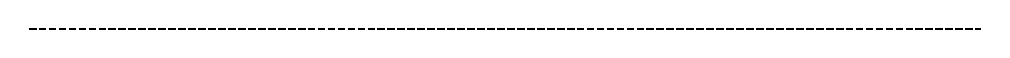
\begin{tikzpicture}
        \draw[dash pattern = on 2.8 pt off 0.8 pt, thick] (0, 0) -- (\linewidth - 1 pt, 0);
    \end{tikzpicture}
\end{center}

\vspace{-0.4cm}

\begin{flushleft}\zihao{5}
    {\calibri \textbf{1. The topics/requirements of the assessment:}}

    {\cambria \textbf{Requirement}

    1. Select a research topic that strongly interests you and your group members

    2. Compose a research paper on the selected topic with your group members

    3. Revise each section of the paper with the teacher and peer feedback}
    \newline

    \textbf{2. Your answer:}
\end{flushleft}

\begin{doublespace}

\begin{center}
    \zihao{5} Abstract
\end{center}

{\zihao{-4}\noindent
This is where you write the abstract.
}
\newpage

\begin{center}
    The title of the paper
\end{center}

This is the introduction of the paper. Note that this part does not need a heading. Also note that the title is not bolded, italicized or underlined. It is in the same font as the rest of the text.

This part usually includes some cites. There are several ways you can do this depending on context (Below we use the famous ``Attention is all you need'' as an example):

\begin{itemize}\tightlist
    \item \citeA{vaswani2017attention} proposed the Transformer model.
    \item In \citeyearNP{vaswani2017attention}, \citeauthor{vaswani2017attention} proposed the Transformer model.
    \item The Transformer model \cite{vaswani2017attention} is widely used in NLP.
    \item In \citeauthor{vaswani2017attention}'s work \citeyear{vaswani2017attention}, the Transformer model was proposed.
    \item For other citation styles, please refer to the documentation of `apacite' package.
\end{itemize}

\section{Methods}

\subsection{Participants}

This part describes the participants of the study.

\subsubsection{This is a subsubsection}

You can include third-level headings if necessary.

\subsubsection{This is another subsubsection}

You can include third-level headings if necessary.

\subsection{Materials}

This part describes the materials used in the study.

\subsection{Procedure}

This part describes the procedure of the study.

\subsection{Data Analysis}

This part describes the data analysis of the study.

\section{Results}

This part describes the results of the study.

Examples of figures and tables are shown in \Cref{Fig:metrics} and \Cref{Tab:metrics}.

For the table, as shown in \Cref{Tab:metrics}, you need a three-line table with the caption on top.

{\setstretch{1.2}
\begin{table}[H]
    \centering
    \caption{The three metrics data for four models}
    \begin{tabular}{c*{4}{>{\centering\arraybackslash}p{1.7cm}}}
    \Xhline{1.2pt}
        \textbf{Model} & \textbf{Deepseek} & \textbf{Llama} & \textbf{Mathstral} & \textbf{Qwen} \\ \hline
        \textbf{Speed (tokens/s)} & 44.3422 & 38.8985 & 33.6797 & 41.4418 \\ 
        \textbf{Confidence} & 0.9193 & 0.972 & 0.9551 & 0.9753 \\ 
        \textbf{Standard Deviation} & 0.92956 & 0.828484 & 0.87568 & 0.45489 \\ \hline
    \end{tabular}
    \label{Tab:metrics}
\end{table}}

For the figure, as shown in \Cref{Fig:metrics}, the caption can be placed both below and above the figure.

\begin{figure}[H]
    \centering
    \caption{The three metrics data for four models}
    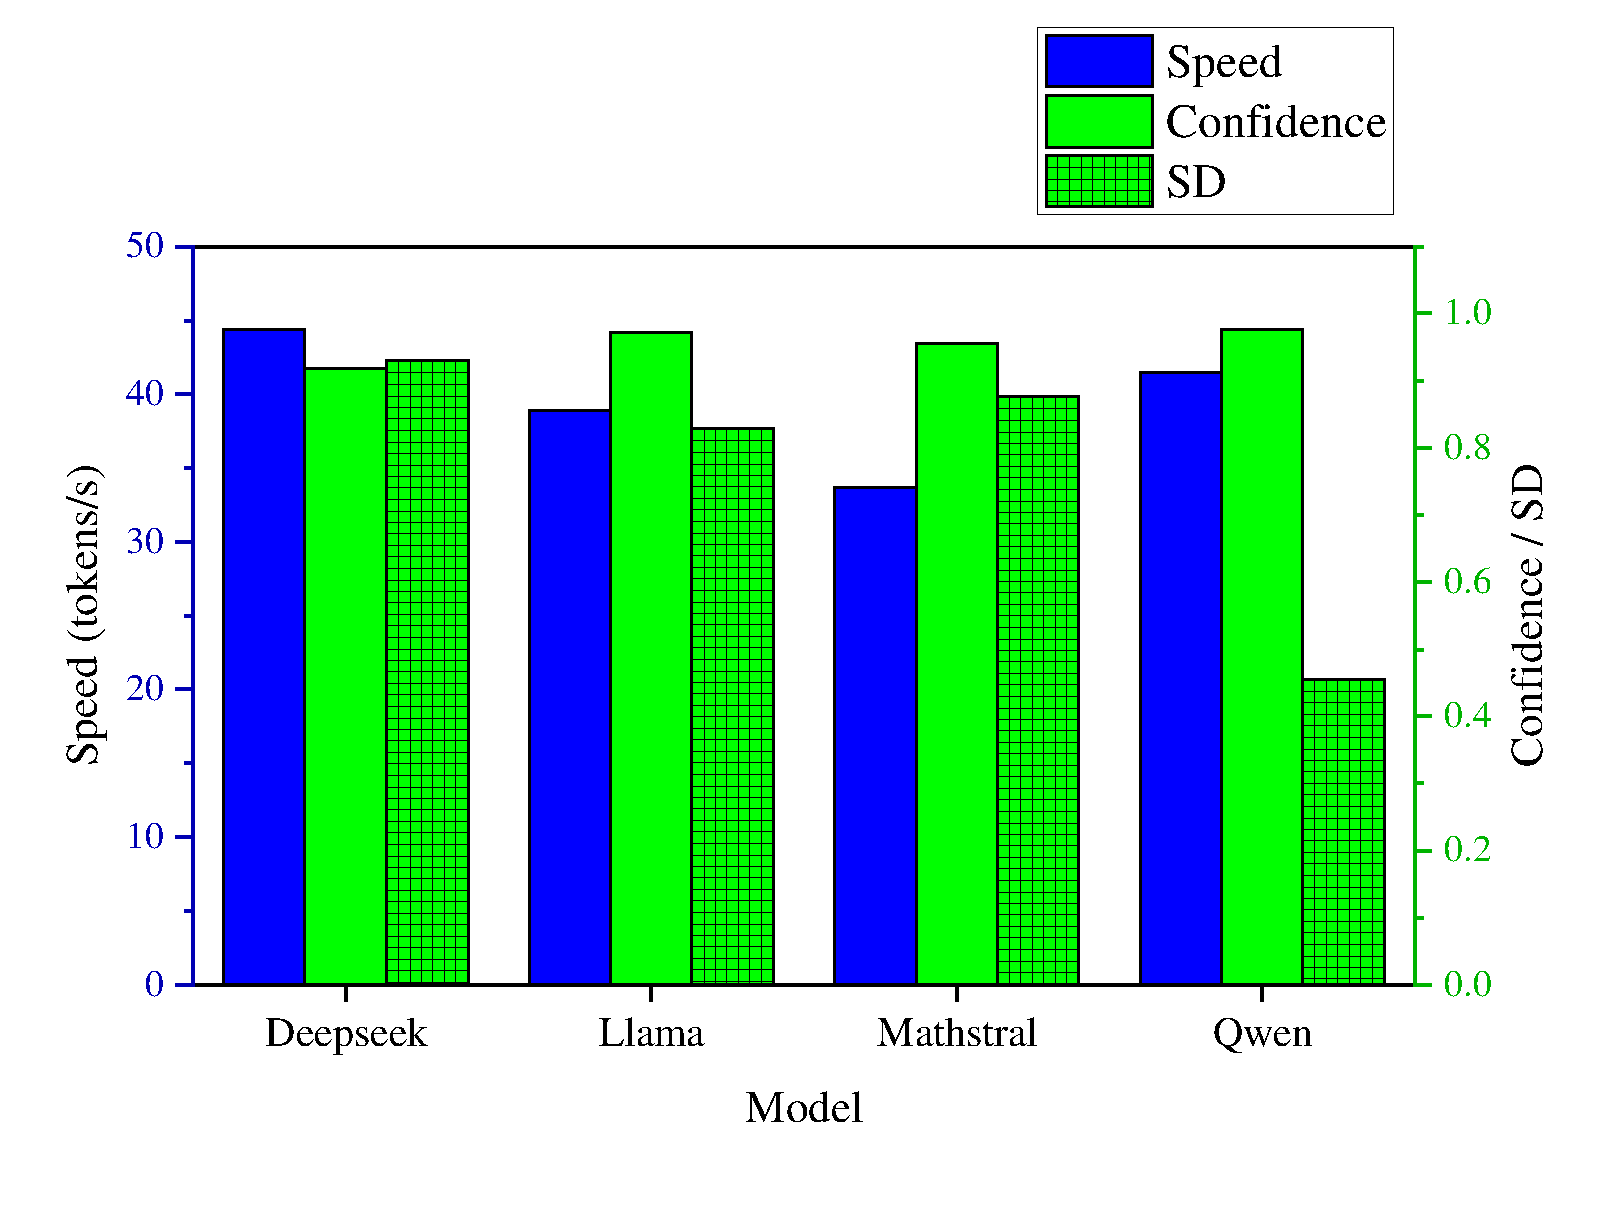
\includegraphics[width=0.9\textwidth]{assets/Metrics.pdf}
    \label{Fig:metrics}
\end{figure}

\section{Discussion and Conclusion}

This part discusses the results of the study and concludes the paper.

\end{doublespace}

\myreferences % 这个命令不会输出任何内容,只是设置了参考文献的格式
\bibliographystyle{apacite}
\bibliography{references.bib}

\end{document}